\section{PIR sensor}

Udgangspunktet for denne undersøgelse er så vidt som muligt at bruge de komponenter vi har til rådighed i Embedded Stock. Hvilket umiddelbart betyder en PIR sensor af typen:

\begin{table}[H] \centering
\begin{tabular}{|p{3cm}|p{11cm}|}
	\hline
	\textbf{Løsning}		
	    & HC-SR501, PIR-bevægelsessensor
	\\ \hline
	\textbf{Producent} 		
	    & Ukendt
	\\ \hline
	\textbf{Interface} 		
	    & TTL\footcite{ttl}
	\\ \hline
	\textbf{Beskrivelse} 	
	    & En PIR-sensor der giver et High output når bevægelse er registeret. High er 3.3 V, og Low er 0 V
	\\ \hline
	\textbf{Krav} 			
	    & Godt kendskab til PSoC creator
	\\ \hline
	\textbf{Fordele}		
	    & Denne PIR-sensor kræver ingen ekstra HW. Justerbar delay og range via potentiometer
	\\ \hline
	\textbf{Ulemper} 		
	    & Begrænset præcision og rækkevidde
	\\ \hline
	\textbf{Pris} 			
	    & Ved lavpris elektronik: 59,- (Hentet gratis på EL-lab)
	\\ \hline
	\textbf{Link} 			
	    & \url{https://www.mpja.com/download/31227sc.pdf} 
	\\ \hline
	\multicolumn{2}{|c|}{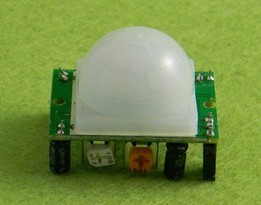
\includegraphics[width=0.3\linewidth]{0_Filer/Figuer/Forudundersoegelse/PIR_sensor_billede.jpg}}
    \\ \hline
\end{tabular}
\end{table}

\subsection{Konklusion}

HC-SR501 PIR-bevægelsessensor opfylder alle de behov der er brug for i vores projekt. Den er lille og kompakt og følsomhed/forsinkelse kan let indstilles. Da sensoren er tilgængelig på Embedded stock, er denne valgt.
